\chapter{Les ondes mécaniques}
Lorsqu'un caillou tombe dans l'eau, l'eau qui se trouve au point d'impact va osciller et cette oscillation va se transmettre à toutes les molécules environnantes et il se forme une onde circulaire. Un bouchon qui flotte à proximité du point d'impact va monter et descendre au passage de la perturbation, mais il ne va pas avancer.

\begin{figure}[ht!]
    \centering
    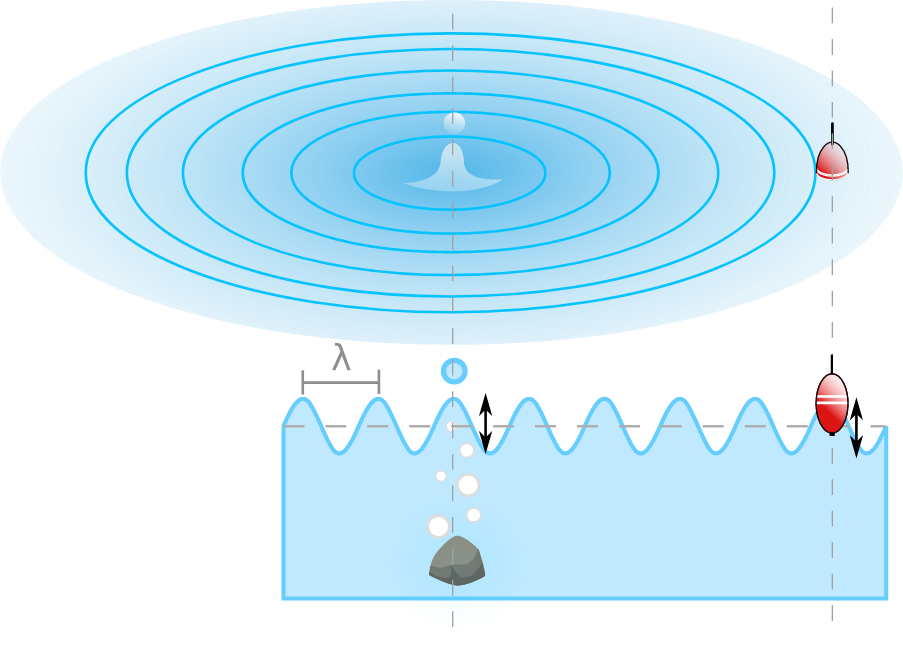
\includegraphics[width=.5 \linewidth]{onde_mecanique.png}
    \caption{Le bouchon à la surface de l'eau.}
    \label{onde_mecanique}
\end{figure}

\newpage

\section{Classification des ondes}
Il existe de nombreux critères sur base desquels classer les ondes mécaniques : milieu de propagation, vitesse, direction de la perturbation. Si on se réfère à la direction de propagation, deux grandes catégories existent :
\begin{itemize}[label=\textbullet]
    \item \motcle{Ondes transversales}
          \pointilles{3}
    \item \motcle{Ondes longitudinales}
          \pointilles{3}
\end{itemize}

\begin{figure}[ht!]
    \centering
    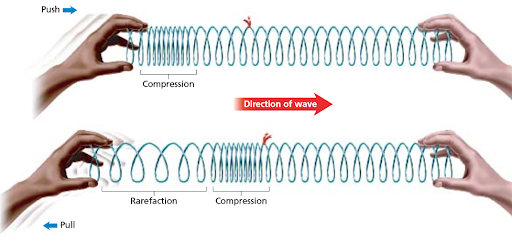
\includegraphics[width=.75 \linewidth]{ondes_longitudinales.png}
    \caption{Un exemple d'onde longitudinale}
    \label{onde_longitudinale}
\end{figure}

\begin{figure}[ht!]
    \centering
    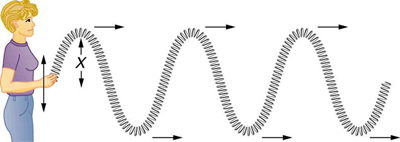
\includegraphics[width=.75 \linewidth]{ondes_transversales.png}
    \caption{Un exemple d'onde transversale}
    \label{onde_transversale}
\end{figure}

\newpage

\section{Vitesse d'une onde}
La vitesse d'une onde mécanique dépend uniquement des propriétés du milieu dans lequel elle circule. Cela implique que cette vitesse ne dépend pas de l'amplitude. En règle générale, plus le milieu est dense, plus la vitesse est élevée.
Si le milieu est homogène, la vitesse de l'onde est constante et les lois du MRU peuvent être utilisées pour connaître les caractéristiques de la perturbation : position, vitesse, durée.

\begin{center}
    \begin{tabularx}{.8 \textwidth}{m{.4 \textwidth} X}
        \hline
        \uppercase{Phénomène} & \uppercase{Vitesse}[m/s]        \\
        \hline
        Son dans l'air        & 340                             \\
        \hline
        Son dans l'eau        & 1500                            \\
        \hline
        Onde sismique         & 4060                            \\
        \hline
        Lumière               & 300 000 000 (\(3 \times 10^8\)) \\
        \hline
    \end{tabularx}
\end{center}


\subsection{Applications}
\begin{enumerate}[a)]
    \item En utilisant la formule de la vitesse moyenne (\(v_{moy}=\frac{\Delta x}{\Delta t}\)) calcule le temps pris par la lumière d'un éclair pour parcourir une distance équivalente à la circonférence de la Terre (\(r_{Terre} = 6400 [ km]\)).
    \item Détermine la distance à laquelle se trouve un orage s'il s'écoule 6 secondes entre la perception de l'éclair et celle du tonnerre sachant que ces deux phénomènes sont simultanés.
\end{enumerate}

\newpage

\section{Onde unique et onde entretenue}
\label{Onde unique et onde entretenue}
Une onde est une perturbation qui se propage. Cette perturbation peut être unique ou se répéter dans le temps. Dans ce cas, l'onde devient une \motcle{onde continue} ou onde entretenue.

\begin{figure}[ht!]
    \centering
    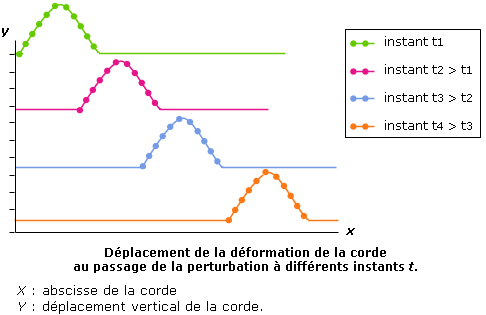
\includegraphics[width=.75 \linewidth]{onde_unique.png}
    \caption{Une onde provoquée par une impulsion unique.}
    \label{onde_unique}
\end{figure}

\newpage

\section{La longueur d'onde}
Pour une onde continue, il existe un nouveau paramètre permettant de les caractériser : leur \motcle{longueur d'onde}.
\begin{itemize}[label=\textbullet]
    \item \motcle{Longueur d'onde}
          \pointilles{3}
\end{itemize}

\begin{figure}[ht!]
    \centering
    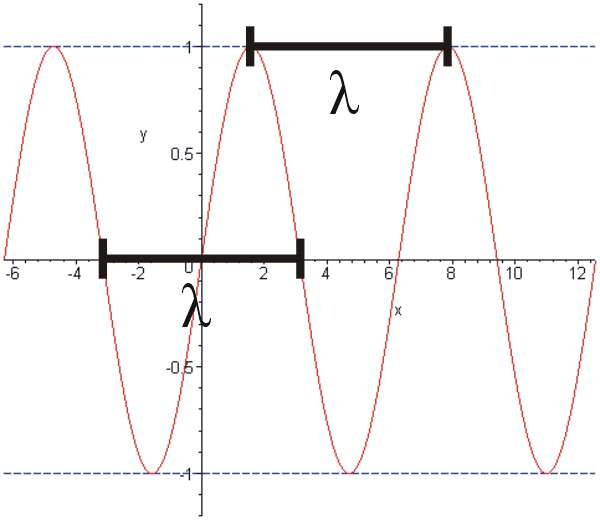
\includegraphics[width=.75 \linewidth]{longueur_onde.png}
    \caption{La longueur d'onde}
    \label{longueur_onde}
\end{figure}

\newpage

\section{Relation fréquence, vitesse, longueur d'onde}
Le schéma ci-dessous représente une onde continue. À partir de ce schéma, établi le lien entre la longueur d'onde, la vitesse et la fréquence de l'onde.
\begin{itemize}[label=\textbullet]
    \item
          \pointilles{2}
\end{itemize}
\begin{figure}[ht!]
    \centering
    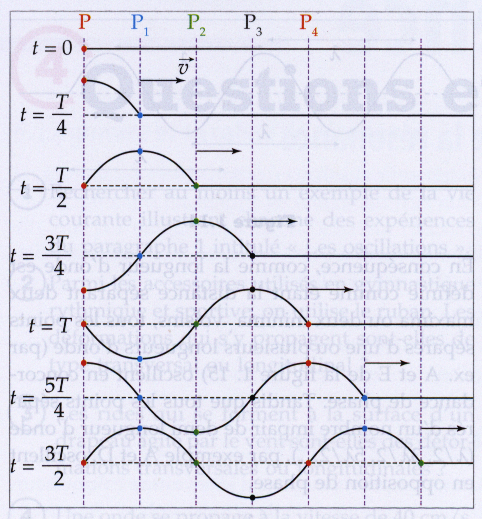
\includegraphics[width=.75 \linewidth]{relation_vitesse_frequence.png}
    \caption{Une onde continue}
    \label{relation_vitesse_frequence}
\end{figure}

Nous avons vu que la vitesse d'une onde dépend des caractéristiques du milieu de propagation. Quel serait, selon toi, l'effet d'une augmentation de la fréquence sur les caractéristiques de l'onde ?

\begin{itemize}[label=\textbullet]
    \item
          \pointilles{2}
\end{itemize}

\section{Élongation d'un point au cours du temps}
Lorsqu'il est atteint par l'onde, chaque point du milieu de propagation se comporte comme un oscillateur harmonique. Nous allons établir l'équation donnant l'élongation en fonction du temps pour un point \(P\) se trouvant à une distance \(x\) de la source \(S\).

\begin{figure}[ht!]
    \centering
    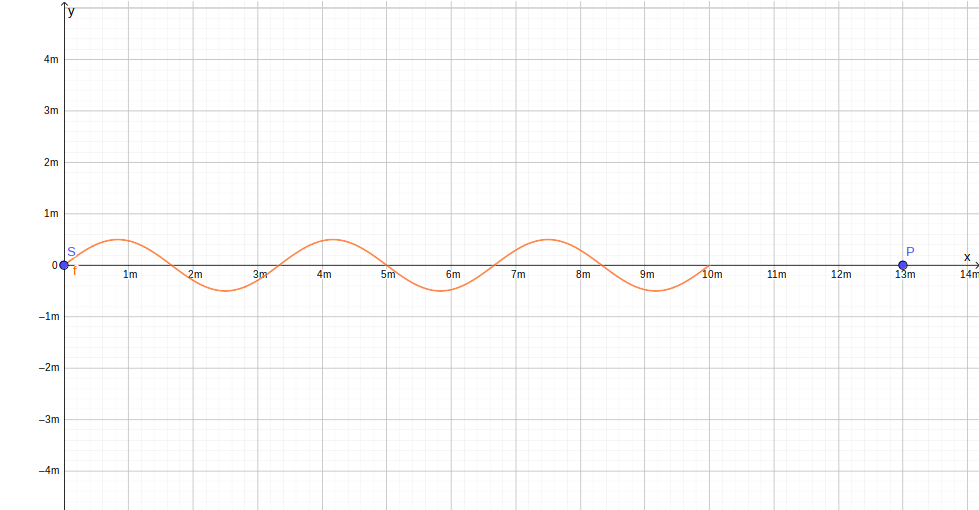
\includegraphics[width=.75 \linewidth]{equation_elongation.png}
    \caption{Élongation en fonction de la distance pour une onde continue.}
    \label{equation_elongation}
\end{figure}

La source se comporte comme un oscillateur harmonique, son élongation est donnée par  \(y_S (t)=A \cdot sin(\omega \cdot t)\).
Si le milieu est homogène, l'élongation du point sera la même que celle de la source, mais avec un décalage dans le temps. On peut donc écrire :
\begin{equation}
    y_P (t + \Delta t)   = y_S (t)
\end{equation}
où \(\Delta t\) est le temps pris par l'onde pour atteindre le point \(P\).
On peut écrire différemment l'équation ci-dessous :
\begin{equation}
    y_P (t)   = y_S (t - \Delta t)
\end{equation}
Le point P se comporte à l'instant \(t\) comme la source se comportait il y a \(\Delta t\) secondes.
On peut donc dire que :
\begin{align}
    y_P (t) & = A \cdot sin (\omega \cdot(t-\Delta t))             \\
    y_P (t) & = A \cdot sin (\omega \cdot t-\omega \cdot \Delta t)
    \label{eqn:position1}
\end{align}
Or, nous savons que \(\Delta t =\frac{x}{v}\). L'équation \ref{eqn:position1} devient alors :
\begin{align}
    y_P (t) & = A \cdot sin (\omega \cdot t-\omega \cdot \frac{x}{v})
    \label{eqn:position2}
\end{align}

Nous savons aussi que \(\omega = 2 \pi \cdot f\), l'équation \ref{eqn:position2} peut donc s'écrire :
\begin{align}
    y_P (t) & = A \cdot sin (\omega \cdot t-2 \pi f \cdot \frac{x}{\lambda \cdot f})
    \label{eqn:position3}
\end{align}

Finalement, on simplifie l'équation \ref{eqn:position3} qui devient :
\begin{equation}
    \tcboxmath[colback=LightBlue,colframe=blue]{y_P (t)= A \cdot sin (\omega \cdot t- \frac{2 \pi  \cdot x}{\lambda})}
\end{equation}

\newpage

\section{La double périodicité des ondes}
\subsection{Périodicité dans le temps}
Dans l'équation de l'élongation en fonction de la position et du temps, si on considère un point fixe, alors le terme \(\frac{2 \pi \cdot x}{\lambda}\) est une constante et l'équation peut s'écrire : \(y_P (t) = A \cdot sin (\omega \cdot t- cst)\). Cela correspond exactement à l'équation d'un mouvement simple harmonique avec une constante de phase égale à : \(\phi = \frac{2 \pi \cdot x}{\lambda}\).

\begin{encadre}
    Chaque point oscille avec la même amplitude et la même fréquence que la source, mais avec un déphasage d'autant plus grand que ce point est éloigné de la source.
\end{encadre}

\subsection{Périodicité dans l'espace}
Si on s'intéresse à l'aspect de l'onde à un instant donné, une photographie de l'onde présentant l'élongation de tous les points alors l'équation de l'onde devient : \(y (x) = A \cdot sin (cst - \frac{2 \pi  \cdot x}{\lambda})\). Cette équation montre qu'à chaque instant l'ensemble des points en oscillation forment une sinusoïde.

\begin{encadre}
    Les ondes continues présentent une double périodicité :
    \begin{itemize}
        \item périodicité dans le temps pour chaque point ;
        \item périodicité dans l'espace pour l'ensemble des points à chaque instant.
    \end{itemize}
\end{encadre}

\newpage

\section{Opposition et concordance de phase}
Sur une onde continue, certains points oscillent de la même manière : ils sont toujours à leur amplitude minimale, maximale ou nulle en même temps. Deux points qui oscillent avec la même élongation sont dits en \motcle{concordance de phase}. Tandis que deux points qui ont toujours une élongation opposée sont dits en \motcle{opposition de phase}.
\begin{itemize}[label=\textbullet]
    \item À quelle condition deux points sont-ils en concordance de phase ?
          \pointilles{2}
    \item À quelle condition deux points sont-ils en opposition de phase ?
          \pointilles{2}
\end{itemize}

\begin{figure}[ht!]
    \centering
    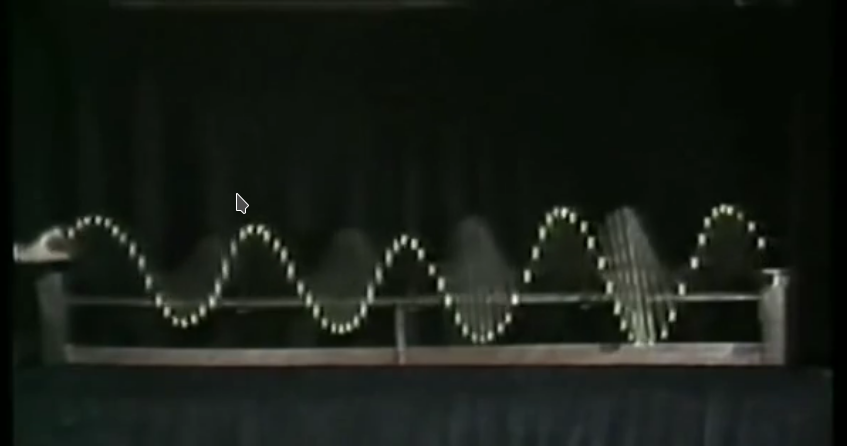
\includegraphics[width=.75 \linewidth]{onde_shive.png}
    \caption{Une onde sur la machine de Shive.}
    \label{onde_shive}
\end{figure}
